\documentclass[a4paper,12pt]{report}

\usepackage[utf8]{inputenc}
\usepackage{graphicx}
\usepackage{listings}
\usepackage{hyperref}
\usepackage{float} % Aggiungi questo pacchetto

\title{Simulatore Distance Vector Routing\\Report per il Progetto di\\Reti di Telecomunicazioni A.A. 2024/2025}
\author{Marco Marrelli}
\date{Dicembre 2024}

\begin{document}
\maketitle

\renewcommand{\contentsname}{Indice}
\tableofcontents{}

\newpage
\section{Introduzione}
Questo progetto riguarda, tramite un simulatore, l'algoritmo di Distance Vector Routing (DVR), un algoritmo utilizzato nel routing sulle reti network.
L'applicazione creata permette di creare e manipolare (con dei limiti prefissati) una rete di router, visualizzarla graficamente e simulare l'esecuzione dell'algoritmo di routing su di essa.
L'output dell'algoritmo (la tabella di routing di ogni router) può essere consultata tramite l'applicazione grafica.

\section{Requisiti}
\begin{itemize}
    \item Python 3.6 (o superiore)
    \item Libreria Tkinter (Framework per la parte Grafica)
    \item Librerie Standard di Python, come:
    \begin{itemize}
        \item typing (per i Type Hints)
        \item math (per Calcoli e Costanti Matematiche)
        \item random (per l'aspetto della Randomicità)
    \end{itemize}
\end{itemize}

\newpage
\section{Struttura della Codebase}
\subsection{Componenti per la Grafica}
\subsection{Componenti per la Logica}

\newpage
\section{Implementazione della Grafica}
\subsection{Visualizzazione Grafica della Rete}
\subsection{Manipolazione della Rete}

\newpage
\section{Parte Logica}
\subsection{L'Algoritmo (Distance Vector Routing)}
Il Distance Vector Routing (conosciuto anche come routing di Bellman-Ford) è un algoritmo di routing dinamico dove ogni router:
\begin{itemize}
    \item Mantiene una tabella delle distanze minime note (vettore) verso ogni destinazione;
    \item Scambia (periodicamente) queste informazioni con i router direttamente collegati ("vicini");
    \item Aggiorna le proprie distanze quando scopre percorsi più brevi attraverso i vicini.
\end{itemize}

\noindent Viene utilizzata l'equazione di Bellman-Ford per calcolare i percorsi ottimali
\[ d_x(y) = \min_v\{c(x,v) + d_v(y)\} \]
\begin{itemize}
    \item $d_x(y)$: distanza minima dal nodo $x$ al nodo $y$;
    \item $c(x,v)$: costo del collegamento diretto tra $x$ e il vicino $v$;
    \item $d_v(y)$: distanza minima dal vicino $v$ al nodo $y$;
\end{itemize}

\noindent Questo approccio permette ai router di selezionare in maniera dinamica la rotta ottimale.
\newpage
\subsection{Implementazione della Logica}
Questo è il codice (semplificato) dell'algoritmo implementato (visualizzabile nel file router.py, nella funzione updateroutes)

\begin{figure}[H] % Modifica l'opzione qui
    \centering
    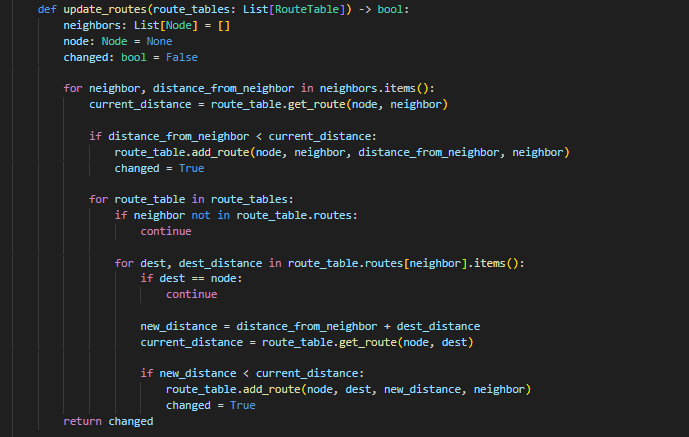
\includegraphics[width=0.9\textwidth]{pseudocode.PNG}
    \caption{router.py::update\_routes() : Pseudocode dell'algoritmo DVR}
    \label{fig:pseudocode.PNG}
\end{figure}

La funzione \texttt{update\_routes} nel file \texttt{router.py} è responsabile dell'aggiornamento delle rotte nel router utilizzando l'algoritmo di Distance Vector Routing.
Di seguito viene fornita una spiegazione dettagliata del funzionamento della funzione:
\begin{itemize}
    \item \textbf{Inizializzazione del Flag}: Viene inizializzato un flag (booleano) \texttt{changed} che viene utilizzato per tracciare se ci sono stati aggiornamenti nelle rotte (\texttt{update\_routes}, riga 13). \\
    Verrà successivamente returnato.
    \item \textbf{Iterazione sui Vicini}: La funzione itera su ogni vicino del router e sulla distanza associata (\texttt{update\_routes}, riga 16). \\
    Per ogni vicino, ottiene la distanza corrente verso di esso dalla tabella di routing (\texttt{update\_routes}, riga 17).
    \item \textbf{Aggiornamento della Rotta Diretta}: Se la nuova distanza verso il vicino è più corta della distanza corrente, la rotta viene aggiornata nella tabella di routing e il flag \texttt{changed} viene impostato a \texttt{True} (\texttt{update\_routes}, righe 20 : 23).
    \item \textbf{Iterazione sulle Tabelle di Routing degli Altri Router}: La funzione itera su ogni tabella di routing degli altri router (\texttt{update\_routes}, riga 26). Se il vicino non è presente nella tabella corrente, viene saltato (\texttt{update\_routes}, riga 27).
    \item \textbf{Iterazione sulle Destinazioni}: Per ogni destinazione e la sua distanza dal vicino, la funzione verifica se la destinazione è il nodo corrente e, in tal caso, la salta (\texttt{update\_routes}, righe 30 : 32).
    \item \textbf{Calcolo della Nuova Distanza}: La funzione calcola la nuova distanza verso la destinazione attraverso il vicino e ottiene la distanza corrente verso la destinazione dalla tabella di routing (\texttt{update\_routes}, righe 35 : 37).
    \item \textbf{Aggiornamento della Rotta Indiretta}: Se la nuova distanza è più corta della distanza corrente, la rotta viene aggiornata nella tabella di routing e il flag \texttt{changed} viene impostato a \texttt{True} (\texttt{update\_routes}, righe 40 : 43).
    \item \textbf{Return del Flag \texttt{changed}}: Come già scritto all'inizio, l'ultima riga di codice riguarda il return del flag \texttt{changed}, per indicare se ci sono stati aggiornamenti nelle rotte (\texttt{update\_routes}, riga 45).
\end{itemize}

\section{Conclusioni}

\end{document}